\section{Volvo Cars architecture framework}\label{sec:VCGAF}

The starting point for defining an architecture framework is to start from the identification of established stakeholders within the domain of the framework. Stakeholders may be individuals, teams,
organizations or classes (of individuals, teams or organizations), while concerns may be fine-grained or very broad in scope~\cite{Emery-Hilliard:2009}. 

%Table \ref{tab:stakeholders} describes the main actors in the challenging scenarios.
% \todo[inline]{elaborate and describe. Also: Include other stakeholders such as customer, driver, ...}

%A suitable electrical architecture needs to take into account the specific needs of each of these stakeholders. 
%In the next section, we will discuss \emph{challenging scenarios} that explore how these stakeholders will interact with the electrical system, its architecture, and its development.

\begin{table}[htb]
\scriptsize
\caption{Overview of Stakeholders}
\label{tab:stakeholders}
\begin{tabular}{rv{0.14\textwidth}v{0.2\textwidth}v{0.26\textwidth}v{0.2\textwidth}}
\toprule
& \textbf{Stakeholder} &	\textbf{Group} & \textbf{Comment} & \textbf{Synonyms} \tabularnewline
\midrule
$\bullet$& Passengers & end-user	\tabularnewline
$\bullet$& Drivers & end-user		\tabularnewline
$\bullet$& Customers & customer & Purchaser of a car or related service & \tabularnewline
$\bullet$& Product planner & customer & Acquirer of electrical system		\tabularnewline
$\bullet$& Purchaser & customer & Purchasers of electrical system		\tabularnewline
$\bullet$& Line managers & management & Has scheduling responsibility, long term quality responsibility, includes group, department	\tabularnewline
$\bullet$& Project managers & management & Owns budget for development	\tabularnewline
$\bullet$& System architects & developers of electrical system & 	\tabularnewline
$\bullet$& Functional developers & developers of electrical system & Owns functional and non-functional aspects & function owner; function realizer; function developer, function realizer, system developer\tabularnewline
$\bullet$& Component developers & developers of electrical system		\tabularnewline
$\bullet$& SW supplier (internal/external) & developers of electrical system	& Can be internal or external from the perspective of the OEM.	\tabularnewline
$\bullet$& HW supplier (internal/external) & developers of electrical system	& Can be internal or external from the perspective of the OEM.	\tabularnewline
%SW supplier (external & developers of electrical system		\tabularnewline
%HW supplier (external) & developers of electrical system		\tabularnewline
$\bullet$& Testers & developers of electrical system		\tabularnewline
$\bullet$& Attribute Owners & developers of electrical system & Owns non-functional attributes like performance	\tabularnewline
$\bullet$& Tool Engineers & developers of electrical system & Specifically testing tools, including design tools (e.g. for requirements)	\tabularnewline
$\bullet$& Calibrators & developers of electrical system & \tabularnewline
$\bullet$& Diagnostic method engineers & maintainers of electrical system		\tabularnewline
$\bullet$& Workshop Personnel & maintainers of electrical system		\tabularnewline
$\bullet$& Fault Tracing Specialists & maintainers of electrical system		\tabularnewline
$\bullet$& Technical Specialist &  specialists &	Support developers and maintainers on specific topics \tabularnewline
\bottomrule
\end{tabular}
\end{table}

Table~\ref{tab:stakeholders} describes the main stakeholders we have identified; they fall into five major groups: 

\begin{itemize}
\item \emph{End-users} of the electrical system, like drivers and passengers.
\item \emph{Customers} stakeholders, such as paying customers of products and services that depend on the electrical system (i.e. the car) and product planners, who acquire the electrical system as part of the overall product.
\item \emph{Management} with responsibility for scheduling, long term quality, groups, departments, and budget.
\item \emph{Developers of the electrical system}  include engineers throughout the value chain that create the electrical system, its architecture, and the necessary tools as well as that test and integrate the various components. 
\item \emph{Maintainers of the electrical system} who interact with the electrical system throughout its lifetime. 
\end{itemize}


Then the identified stakeholders motivate the set of concerns on which the architecture framework will focus.
This will help the consumer of the architecture framework and of the views and connected modeling tools to understand why
they are modeling and when they are done.
In order to define the stakeholders concerns we identified a set of challenging scenarios through a number of workshops for elicitation and validation. 
Figure~\ref{fig:challenging-scenarios} gives an overview of the scenarios that are strongly connected to the viewpoints we will detail in this paper. These scenarios are described in the following items. \patrizio{Ensure that there is a mapping between these scenarios and the viewpoints we will discuss. Indeed we need to consider also SoS from WP3}

\begin{figure}[htb]
\begin{center}
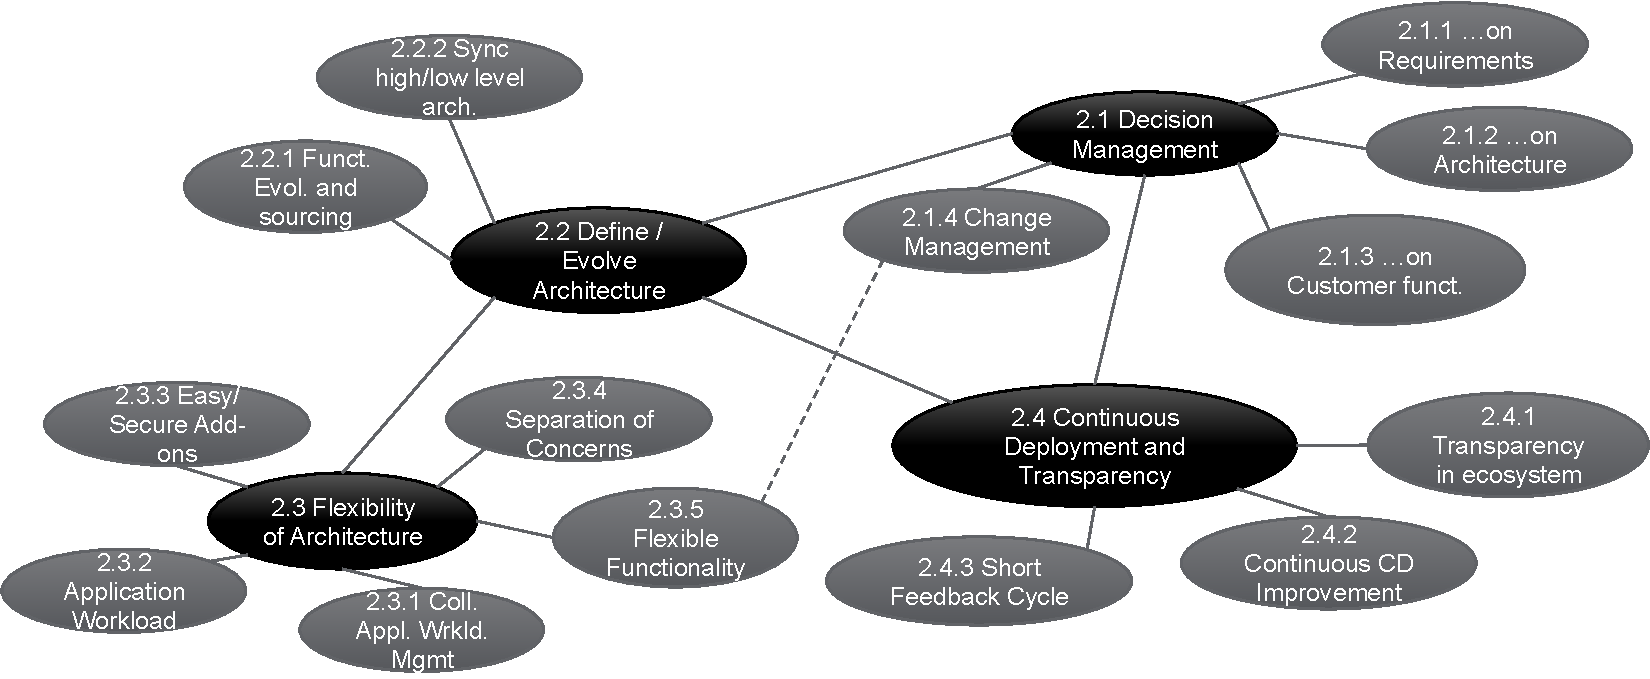
\includegraphics[width=\textwidth]{figures/challenging-scenarios} 
\caption{Overview of challenging scenarios}
\label{fig:challenging-scenarios}
\end{center}
\end{figure}


\begin{itemize}
\item Scenario 2.1 {\bf decision management } aims at exploring how to make, communicate, and manage decisions. 

\begin{quote}
{User Story:} \emph{``As a member of the development ecosystem I would like to have a clear understanding on how to take decisions and how to communicate them.''}
\end{quote}


Interesting sub-scenarios include decisions about:

\begin{itemize}
\item  {\em Requirements (2.1.1)}: When decisions on requirements are made too early, it will lead to unnecessary changes.

%\textbf{Trigger:} Requirement needs to be refined so that others can continue working.

\begin{quote}
{User Story:} 
\emph{``As a component responsible, I need to write a requirement. 
Currently, I am forced to write the requirement in a certain document or certain structure. 
This determines whether the requirement refers to a hw or sw component, whether it will be implemented in-house or by an external supplier. 
Often, it is too early to make such decisions and changes are necessary later, when more information becomes available. 
I do not feel comfortable to make this decision so early.''}
\end{quote}

\item {\em Architecture (2.1.2)}: Architectural decision making involves making the right decision, communicating it, ensuring that it is followed, and changing it when needed. 

%\textbf{Trigger:}  Architectural decision required (it is beneficial and possible). 

\begin{quote}
{User Story:} 
\emph{``As an architect} (one of \{system architect; functional developer; low level architect\})\emph{, I need to make the right decision at the right moment (i.e. when it is useful to make the decision and when the necessary information is available).  
I need to make this decision on the right level. 
I need to be introvert to make the best possible decision on the available data and extrovert to communicate it.''}
\end{quote}

\item {\em Customer functions (2.1.3)}:  Electrical architecture is guiding realization of customer functions, but it is not obvious how the architecture support customer functions (with respect to tracing and methodology).

%\textbf{Trigger:}  Decision about customer function required. 

\begin{quote}
{User Story:} 
\emph{``As a product manager, I want to be supported by the electrical architecture in making decisions about customer functions. Based on a wishlist from the Market Analysis Department, I engage in a dialog with the departments that design the system. 
For this task, I wish for support from an electrical architecture that not only takes into account non-functional aspects, but also the nature of customer functions (which changes over time).''}
\end{quote}

\item {\em Change management (2.1.4)}: Good flexibility of the architecture allows to continuously remove assumptions and do changes even late in the process. 
However, in a weak electrical architecture, such changes will impact the stability of the electrical system because of technical dependencies. 

\begin{quote}
{User Story:} 
\emph{``As a product planner I want to have a flexible Change Management process, allowing me to change or add functions late in the process, often with the goal of removing assumptions. 
This includes for example defining and changing the allocation of Functions to ECU late in the process.''}
\end{quote}
\end{itemize}
 
 
\item Scenario 2.2 {\bf define/evolve architecture} explores aspects of long-time evolution of the electrical architecture.
This includes:

\begin{itemize} 
\item {\em The impact of long-term sourcing decision on the logical architecture (2.2.1)}: Long term sourcing contracts allow to optimize production cost, but constraint evolution of the architecture. 
\begin{quote}
{User Story:} 
\emph{``As a Function Developer I want to optimise the evolution of functions without considering sourcing agreements. 
Today I have to discuss with the product planner about the plan for a function two years or more in advance to reflect on existing contracts, e.g. when related nodes are sourced for different time intervals. Problem: Sourcing needs make physical layout dominate logical decisions.''}
\end{quote}

%Architectural frameworks such as AUTOSAR can support functional evolution on component level, but addressing this scenario would also require more  thinking on how to support moving around functions on high level architecture.

\item {\em The danger of architecture and design  evolving in different directions (2.2.2)}: If not actively managed,  architecture and design diverge over time. 
The architecture is then perceived as outdated and not useful, thus it looses its ability to guide design decisions and implementation.

\begin{quote}
{User Story:} 
\emph{``As a system architect or function developer I want a stringent correlation between architecture and design. Otherwise, one or the other is wrong. ''}
\end{quote}
\end{itemize}

\item Scenario 2.3 {\bf flexibility of architecture} addresses different scenarios that emphasize flexibility of the electrical architecture, both on a technical and on a process level. On a technical level, more capacity in the ECUs allows to add functionality late. 
On a process level, the available resources need to be managed across several contributing partners.
This includes:

\begin{itemize}
\item {\em application workload management from a process perspective (2.3.1)}: 
\begin{quote}
{User Story:} 
\emph{``As a functional developer, I want to be flexible when it comes to application workload. 
Suppliers should be able to acquire and return resources dynamically throughout the lifecycle. ''}
\end{quote}
\item {\em application workload management from a technical perspective (2.3.2)}: higher capacity of ECUs and Buses will facilitate late or even very late updates (i.e. when the vehicle is on the street), because new functionality could use more resources.
This flexibility comes at a cost and it is not trivial to understand where the break-even point is.

\begin{quote}
{User Story:} 
\emph{``As a system architect I want to balance capacity of ECUs and Buses against cost.''}
\end{quote}

\item {\em easy and secure add-ons (2.3.3)}: being able to add new functions in a secure and easy way would allow to detach software development to some extend from the development cycle. 
During the development of a car, an OEM could focus on the critical basic functionality. 
Convenience features as well as more advanced connected features could be added independent from the start of production.
This would allow to develop more continuously and should decrease the peak of trouble reports before critical deadlines observed earlier~\cite{modelsward13}.

\begin{quote}
{User Story:} 
\emph{``As a  functional developer I want to be able to add new functions (very) late. Such add-ons could originate from third parties and should be added even after the vehicle has been put into use. ''}
\end{quote}

\item {\em separation of concerns (2.3.4)}: 
\begin{quote}
{User Story:} 
\emph{``As a system architect, I want to balance separation of concerns on two levels: between domains (e.g. safety vs. infotainment) and levels of abstractions (e.g. architecture vision vs architecture implementation).''}
\end{quote}

\item {\em flexible functionality (2.3.5)}:
\begin{quote}
{User Story:} 
\emph{``As a functional developer, I want to be flexible about the functions that are running in the car and allow for very late deployment. ''}
\end{quote}
\end{itemize}
 
\item Scenario 2.4 {\bf continuous deployment and transparency} includes:

\begin{itemize}
\item {\em the need for openness and transparent information through out the different value chains in the automotive ecosystem (2.4.1)}: Good transparency in the value chain supports flexibility, since all partners can take appropriate action to reach a (changing) goal quickly. 
The \emph{cone of uncertainty} is a good example for this~\cite{cone-of-uncertainty,cone-of-uncertainty2}: In the beginning of a project, not much data is available and decisions are very uncertain. 
As the project proceeds, assumptions are removed and uncertainty is reduced, but as  a consequence, it becomes harder to make decisions that change a lot. 
Good transparency can help to reduce the uncertainty quicker and can allow to decide fast in order to learn fast.

\begin{quote}
{User Story:} 
\emph{``As any developer of the electrical system (internal or external), I want to have access to relevant decision, to the status of relevant assumptions, and knowledge generated during the development. 
This allows me to participate in the fast learning throughout the value chain and enables me to be effective and flexible in my work.''}
\end{quote}

\item {\em the need for using this information to continuously improve an continuous integration, delivery, and deployment flow (2.4.2)}: 
Cross-organizational continuous integration, delivery, and deployment facilitates fast feedback and rich learning.
This learning should also help to improve the interaction of organizations and the integration flow between them.

Have a culture of continuous improvement between VCC and partners	Apply Continuous Deployment to the CD tool chain

\begin{quote}
{User Story:} 
\emph{``As a Project Manager, I want to have a culture of continuous improvement within the OEM and with partners in the value-chain. As any developer of the electrical system (internal and external) I want to benefit from and take responsibility in improving the continuous delivery flow.''}
\end{quote}

\item {\em the need for establishing short feedback cycles (2.4.3)}: While developing new functionality, basic software, and hardware, one should plan on how to receive feedback, which data to collect, and how to use it in the development.

\begin{quote}
{User Story:} 
\emph{``As any developer of the electrical system (internal or external) I want to have quick feedback on how my contribution will work on the various levels of integration. 
As a Functional Developer, I want to have fast and defined feedback cycles. 
As a tester, I want quick updates on all levels of tests and continuous improvement of functionality.''}
\end{quote}
\end{itemize}

\end{itemize}

\patrizio{We need to add scenarios for the System of Systems part; unfortunately this is a bit decoupled in NGEA but we can recover that from WP3}
The identified architecture-related concerns determine the choice of viewpoints and view to be included. 
It is important to note that almost each viewpoint detained in the following is already handled within the current architecture of Volvo Cars. However, we are investigating the definition of proper viewpoints that will create the architecture framework. %of the
%Viewpoints are the principal content of an architecture framework. In fact the viewpoint defines the conventions and establishes the basis for interpreting views. Moreover, ``{\em each viewpoint establishes the notations, models, techniques and methods to be used in architecture descriptions resulting from applying the framework.}"~\cite{Emery-Hilliard:2009}.
\patrizio{here we have to explain that there are the viewpoints in the litareture, other important viewpoints for Volvo Cars, but that in this paper, due to space restrictions we only focus on three viewpoints}
Therefore, in addition to the viewpoints summarized in Section~\ref{sec:AAF} we foresee the following viewpoints:
	\begin{itemize}
	\item \emph{Continuous integration and deployment} (detailed in Section~\ref{sec:CIDviewpoint}) - OEMs are increasingly interested to reduce the development time, to increase flexibility, to have early feedback on decisions made, and to add new functionalities incrementally even after production. %However, another trend is the rapid development of more advanced active safety systems that require \del{a} special handling.\eric{does the last point here not relate more to connected cars and safety?}
	\item \emph{Connected cars and safety} (detailed in Section~\ref{sec:SoSviewpoint}) - Future scenarios of collaborating autonomous vehicles, like platooning, will require to extend the vehicle safety architecture across the classical boundaries of single vehicles and will ask for an open and adaptive architecture able to support runtime assessment of safety. 
	\item \emph{Security and privacy of connected cars} - Connected cars open new important challenges from the point of view of security and privacy.
	\item \emph{Ecosystem and transparency} - related to the value net viewpoint of AAF~\cite{TUM-I0915,Broy}. %activities of, and the dependencies between the stakeholders of the end-toend value creation process which happens within a specific value net. 
	The ecosystem around the OEM can be seen as a virtual %A value net is defined as a virtual
organization consisting of the OEM, its suppliers and other partners %and other constituents 
involved in the process of creating customer value.
	\item \emph{Autonomous cars} - autonomous cars require special architecture solutions, e.g. inspired to autonomous and self-adaptive systems~\cite{Salehie2009}.
	\item \emph{Modes management} - a mode viewpoint is needed to design the different modes of a vehicle as well as the transitions from one mode to another.
	\item Special viewpoints and views might be conceived to enable dissemination and communication of the architecture to developers and other stakeholders.
	\end{itemize}

%In order to define the viewpoints we use a template similar to the one suggested in~\cite{Yania}:
%\begin{itemize}
%\item Definition: Definition of the viewpoint is presented.
%\item Stakeholders: Although the stakeholders are not explicitly identified for the viewpoints
%in the AAF and ADF, we list the stakeholders.
%\item Concerns: Stakeholder concerns are defined.
%\item Views: The views governed by the viewpoints are presented.
%\item Model kinds: The model kinds used in the viewpoint are presented.
%\end{itemize}



The natural consequence of the use of multiple viewpoints and views in architecture
descriptions is the need to express correspondences and consistency rules between those views.
The mechanisms introduced in~\cite{42010} is called model correspondences and it allows the definition of relations between
two or more architecture models. Since architecture views are composed of architecture models~\cite{42010}, model correspondences can be used to
relate views to express consistency, traceability, refinement or other dependencies~\cite{Emery-Hilliard:2009}.
These mechanisms allow an architect to impose constraints between types of models and then demonstrate that them
are satisfied by the architecture. 



%
%
%
%Architecture descriptions take many forms and
%serve many purposes throughout the life cycle of development,
%operation and maintenance activities. The use of {\em multiple views}
%- diverse representations for distinct audiences and uses - has
%been a major tenet of architecture description since the earliest
%work in software architecture. 
%The use of multiple views has become standard practice
%in industry~\cite{4+1,ICSE2010,42010}. A survey recently conducted
%on the industrial needs from architectural languages~\cite{whatindustrywants} (see Section~\ref{sect:survey})
%revealed that 85\% of the 48 interviewed practitioners use
%multiple views when architecting a software system, with
%a total of nine different views and a predominant use of
%structural, behavioral, and physical views reported. 


\section{Continuous integration and deployment viewpoint}\label{sec:CIDviewpoint}
\patrizio{Magnus, Eric, Rogardt}

\subsection{Overview}
Agile approaches and practices such as continuous integration and deployment promise to help reducing development time, to increase flexibility, and to generally shorten the feedback cycle time. However, 
the  complex supplier network,
and typical setup with a large number of ECUs,
pose specific challenges to %\chg{agile development methods, and specifically 
%with respect 
%to continuous integration and deployment of software.}{
these practices. %}.

First,  dependencies between ECUs raise multiple concerns,
regarding organization, versioning and testing:
(i)  organization -
%the question is related to who should be 
identifying the recipient
of a given software change; (ii)
 versioning -
the question is related to the compatibility of the software version of specific ECUs; and
% software
%that are compatible.
(iii)  testing -  %This then carries over to the testing effort,
compatible combinations need to be validated. 
Second, support for continuous deployment has to face with safety concerns.
%relates to the connectivity of ECUs. 
%the extent of this, in turn, raises not least security concerns.
Should, for instance, the software of an ECU responsible for a safety critical function
be modifiable at runtime?

Dependencies between ECUs are a property of the architecture.
As mentioned, the emergent architecture may differ from the intended architecture,
and continuous integration and deployment of software may entail architectural changes.
This highlights both the need for collaboration % touches on the concern of the need for collaboration
between parts of the organization working on different architectural levels, and the need of a proper support
for agile and flexible architecting.
%Furthermore, the architectural framework should support agile architecting.

Addressing these concerns suggests
two architectural views and viewpoints:
(i) one covering architecture as an enabler
of continuous integration and deployment,
facilitating variant handling and coordination of updates, and
%
(ii) another considering continuous integration and deployment
on the architecture level,
facilitating reasoning about modifications to the architecture itself.

\subsection{Concerns}
\patrizio{A listing of the architecture-related concerns framed by this viewpoint. This is
crucial information for the Architect, because it helps her decide whether this
viewpoint will be useful to apply to a given system of interest, and to
communicate with its stakeholders.}

\subsection{Anti-concerns}
\patrizio{Optional. It can be useful to document the kinds of issues a viewpoint is not
appropriate for. Articulating anti‐concerns may be a good antidote for certain
overly used notations.}

\subsection{Typical stakeholders}
\patrizio{Optional. The typical audiences for views prepared using this viewpoint. Who
are the usual stakeholders for this kind of view?}

\subsection{Model languages}
\patrizio{For each type of model used, describe the language or modeling techniques to
be used. Each model language is a key modeling resource that the viewpoint
makes available. Model languages provide the vocabularies for constructing the
view. ISO/IEC 42010 does not specify how a modeling language is documented.
It could be by reference to an existing modeling language (e.g., EAST-ADL or UML)
or technique (e.g., M/M/4 queues); by providing a metamodel for the language
to define the language's core constructs; via a template that users fill in; or by
some combination of these methods.}

\subsection{Model correspondence rules}
\patrizio{The viewpoint may specify model correspondence rules. Each one may be
documented here.}

\subsection{Operations on views}
\patrizio{Operations define the methods which may be applied to views and their
models. Operations can be divided into categories: Creation methods are the
means by which views are prepared using the viewpoint. These could be in the
form of process guidance (how to start, what to do next); or work product
guidance (templates for views of this type); heuristics, styles, patterns, or other
idioms. Interpretive methods provide the means by which views are to be
understood by readers and system stakeholders. Analysis methods are used to
check, reason about, transform, predict, apply and evaluate architectural
results from this view. Implementation methods capture how to realize or
construct systems using information from this view.}

\subsection{Examples}
\patrizio{Optional. This section provides examples for the reader.}

\subsection{Sources}
\patrizio{What are the sources for this viewpoint, if any? This may include author,
history, literature references, prior art, etc.}

\section{System of Systems: vehicle point of view}\label{sec:SoSviewpoint}
\patrizio{Piergiuseppe, Patrizio.}

\subsection{Overview}
Connected cars will benefit from Intelligent Transport Systems (ITS), Smart Cities and IoT to provide new application scenarios like smart traffic control,  smart platooning coordination, collective collision avoidance, etc. 
Vehicles will combine data collected through its sensors %from the inside vehicle 
with external data coming from the environment, e.g. other vehicles, road, cloud, etc. %In such scenario, different applications will be possible: smart traffic control, better platooning coordination and enhanced safety in general. 
%While solving congestion is undoubtedly beneficial, safety remains the top priority for OEMs.

%In connected vehicles, safety aspects become more complex. 
Connected vehicles will face new challenges and opportunities related to safety issues.
%On the one hand, c
Current %While there are clear 
regulations for safety aspects, like the ISO 26262 standard, do not account for scenarios in which the %provide a clear regulation for  
% regarding isolated car system (seat belts, airbags etc..) like in the safety standard ISO 26262, there is a lack of 
%safety requirements for 
%systems of connected cars. The 
vehicle is part of a more complex system; the challenge is on how to manage new hazards that coming from the environment could jeopardize safety. 
%The core ECUs of the car (in charge of braking, steering, engine control, etc.) are part of a closed system in which all the safety requirements can be certified at design time. Exposing these crucial components to the outside environment would invalidates the assumptions that have been made so far. In fact, manufactures have preferred to limit the interfaces of the communication infrastructure due to the enormous hazard potential. In a connected world,  this is no longer possible. Sharing and controlling sensitive information could be crucial in dangerous situations. 
%On the other hand, c
At the same time, connected cars open new opportunities for safety, called ``connected safety" within Volvo Cars\footnote{\url{https://goo.gl/mIWWS3}}: %({\small \url{https://goo.gl/mIWWS3}}):
e.g., this new technology will allow a connected car to be aware of a slippery road, of cyclists on the road, etc., so to initiate all the actions needed to avoid accidents and collisions. 
%
%after it has been informed by another car and the information has been propagated via the Volvo Cloud. In such scenario, the informed car could automatically slow down reducing the risk for potential accidents. 

These scenarios are posing new requirements to the architecture. %To deal with similar scenarios, changes need to be made in the architecture. 
We foreseen two different viewpoints and views: (i) %one viewpoint and view showing the architecture 
from the point of view of a single connected car, which has to offer the functionalities needed to realize the scenario, and (ii) %another viewpoint and view representing the 
from the point of view of the system of systems  (i.e. cars connected with other entities of their environment), spanning from the agreements between the different systems affected, e.g. different OEMs, cloud providers, road infrastructures, etc., to the definition of the scenario that the system of systems has to realize, like the slippery road mentioned above. 

% agreements between the different systems affected. In order to achieve the proper behavior of such system different stakeholders must be involved. From tier 1 and tier 2 suppliers to the cloud provider, they all have to agree on common interfaces and safety guarantees that must be respected.

%The core ECUs of the car (in charge of braking, steering, engine control, etc.) are part of a closed system in which all the safety requirements can be certified at design time. Exposing these crucial components to the outside environment would invalidates the assumptions that have been made so far. In fact, manufactures have preferred to limit the interfaces of the communication infrastructure due to the enormous hazard potential. In a connected world,  this is no longer possible. Sharing and controlling sensitive information could be crucial in dangerous situations. 

%Until lately, safety has been dedicated in surviving crashes, with the emerging connected vehicle it will be about avoiding them. For example, the new technologies developed by Volvo allow a connected car to be aware of a slippery road after it has been informed by another car and the information has been propagated via the Volvo Cloud. In such scenario, the informed car could automatically slow down reducing the risk for potential accidents.

%To accomplish similar scenarios, radical changes need to be made in the architecture descriptions and agreements between the different systems affected. In order to achieve the proper behavior of such system different stakeholders must be involved. From tier 1 and tier 2 suppliers to the cloud provider, they all have to agree on common interfaces and safety guarantees that must be respected.

%<<<<<<< HEAD
In general, the main issue with safety guarantees in connected cars is that a full analysis of the system is not possible at design time. When moving from a single vehicle to a cooperative system, a new safety analysis is required to handle uncertainties at runtime. Some approaches have been proposed to deal with certification at runtime, e.g.~\cite{runtime1, runtime3}, but a clear framework that can be used to define the connected safety requirements is still missing.
%=======
%The main issue with safety guarantees in connected cars, is that a full analysis of the system is not possible at design time. When moving from a single vehicle to a cooperative system, a new safety analysis is required to handle the uncertainties at runtime. Therefore, in order to benefit from the collaborative system, is necessary to move some of the safety analysis from design time to runtime. Some approaches have been proposed to deals with certification of the safety guarantees at runtime \cite{runtime1}, \cite{runtime2}, \cite{runtime3}, but there is still not a clear framework utilized to define the connected safety requirements.
%>>>>>>> 4ffb434a25eb0042a3685e7d03d264e7c0eb62b1

\subsection{Concerns}
\patrizio{A listing of the architecture-related concerns framed by this viewpoint. This is
crucial information for the Architect, because it helps her decide whether this
viewpoint will be useful to apply to a given system of interest, and to
communicate with its stakeholders.}

\subsection{Anti-concerns}
\patrizio{Optional. It can be useful to document the kinds of issues a viewpoint is not
appropriate for. Articulating anti‐concerns may be a good antidote for certain
overly used notations.}

\subsection{Typical stakeholders}
\patrizio{Optional. The typical audiences for views prepared using this viewpoint. Who
are the usual stakeholders for this kind of view?}

\subsection{Model languages}
\patrizio{For each type of model used, describe the language or modeling techniques to
be used. Each model language is a key modeling resource that the viewpoint
makes available. Model languages provide the vocabularies for constructing the
view. ISO/IEC 42010 does not specify how a modeling language is documented.
It could be by reference to an existing modeling language (e.g., EAST-ADL or UML)
or technique (e.g., M/M/4 queues); by providing a metamodel for the language
to define the language's core constructs; via a template that users fill in; or by
some combination of these methods.}

\subsection{Model correspondence rules}
\patrizio{The viewpoint may specify model correspondence rules. Each one may be
documented here.}

\subsection{Operations on views}
\patrizio{Operations define the methods which may be applied to views and their
models. Operations can be divided into categories: Creation methods are the
means by which views are prepared using the viewpoint. These could be in the
form of process guidance (how to start, what to do next); or work product
guidance (templates for views of this type); heuristics, styles, patterns, or other
idioms. Interpretive methods provide the means by which views are to be
understood by readers and system stakeholders. Analysis methods are used to
check, reason about, transform, predict, apply and evaluate architectural
results from this view. Implementation methods capture how to realize or
construct systems using information from this view.}

\subsection{Examples}
\patrizio{Optional. This section provides examples for the reader.}

\subsection{Sources}
\patrizio{What are the sources for this viewpoint, if any? This may include author,
history, literature references, prior art, etc.}

\section{Ecosystem and transparency viewpoint}
\patrizio{Magnus, Eric, Rogardt}

\subsection{Overview}

\subsection{Concerns}
\patrizio{A listing of the architecture-related concerns framed by this viewpoint. This is
crucial information for the Architect, because it helps her decide whether this
viewpoint will be useful to apply to a given system of interest, and to
communicate with its stakeholders.}

\subsection{Anti-concerns}
\patrizio{Optional. It can be useful to document the kinds of issues a viewpoint is not
appropriate for. Articulating anti‐concerns may be a good antidote for certain
overly used notations.}

\subsection{Typical stakeholders}
\patrizio{Optional. The typical audiences for views prepared using this viewpoint. Who
are the usual stakeholders for this kind of view?}

\subsection{Model languages}
\patrizio{For each type of model used, describe the language or modeling techniques to
be used. Each model language is a key modeling resource that the viewpoint
makes available. Model languages provide the vocabularies for constructing the
view. ISO/IEC 42010 does not specify how a modeling language is documented.
It could be by reference to an existing modeling language (e.g., EAST-ADL or UML)
or technique (e.g., M/M/4 queues); by providing a metamodel for the language
to define the language's core constructs; via a template that users fill in; or by
some combination of these methods.}

\subsection{Model correspondence rules}
\patrizio{The viewpoint may specify model correspondence rules. Each one may be
documented here.}

\subsection{Operations on views}
\patrizio{Operations define the methods which may be applied to views and their
models. Operations can be divided into categories: Creation methods are the
means by which views are prepared using the viewpoint. These could be in the
form of process guidance (how to start, what to do next); or work product
guidance (templates for views of this type); heuristics, styles, patterns, or other
idioms. Interpretive methods provide the means by which views are to be
understood by readers and system stakeholders. Analysis methods are used to
check, reason about, transform, predict, apply and evaluate architectural
results from this view. Implementation methods capture how to realize or
construct systems using information from this view.}

\subsection{Examples}
\patrizio{Optional. This section provides examples for the reader.}

\subsection{Sources}
\patrizio{What are the sources for this viewpoint, if any? This may include author,
history, literature references, prior art, etc.}